% ====================== THE TEXT FILE ===========================

%%    In this file you insert your data -from title to author to references - all the text etc you need for your poster!
%%    You may rename it, but be sure to adjust the name in the setting-file.
%%    If you really have to, you can change the size and color of your text in this file at the beginning of every text frame. The standard size for text is \Large.

% ====================== POSTER COLOR ===========================

%% Choose the color of your poster. You have various possibilities, pick one from the list below and insert it in the \def- brackets, standard for colored background is "ETH5"
%% If you want to have a poster with --- white background ---, please choose a different template for SETTING your tex-file  =>  "Poster-portrait-white.tex" OR "Poster-landscape-white.tex"

\definecolor{ETHBlue}{RGB}{33,92,175}		% blue  
\definecolor{ETHGreen}{RGB}{98,115,19}		% green
\definecolor{ETHPurple}{RGB}{163,7,116}		%  purple for whole page !!
\definecolor{ETHGray}{RGB}{111,111,111}		% gray
\definecolor{ETHRed}{RGB}{183,53,45}		% red
\definecolor{ETHPetrol}{RGB}{0,120,148}		% green/blue 
\definecolor{ETHBronze}{RGB}{142,103,19}	% bronze



\def\linecolor{verylightgray} %%% don't change, necessary for white and colored posters


% ===========Choose your COLOR here or change it to WHITE  ===========================

 %\def\postercolor{ETH5} %%% standard for COLORED posters

\def\postercolor{white} % if your poster has a WHITE background, please define the following parameters as well. Otherwise just command them out
\def\backgroundcolortitle{ETHBlue} %%% backgroundcolor of the title box
\def\backgroundcolorcolor{verylightblue}%%% backgroundcolor of the introduction and conclusion boxes
\def\backgroundcolorwhite{verylightgray}%%% backgroundcolor for the rest of the boxes




% ======================   POSTER CONTENT ! =====================================

% your first information - will appear as title, author(s), affiliation, partner/sponsors

% ====================== ORGANISATIONAL UNIT ===================
%%your department
\def\department{\linespread{1.1}
\Large Organisational unit,\\
can be spread over 2 lines
}%%% you may have to adjust the position of the text in the setting file, line 102 -> \hspace{}

% ====================== TITLE ===========================
\def\title{
\VERYHuge \white {\bf %%%%
Title of the poster, as brief and concise %\\[20pt] % try out where you can seperate your title best, especially for changes of poster direction - portrait or landscape
as possible  \\[20pt] 
- but still interesting
}
\\[20pt]}


% ====================== AUTHORS ===========================
%% authors
\def\authors{\LARGE Author one$^1$, Author two$^2$,...}

% ====================== AFFILIATION ===========================

%% affiliations - fill in and extend when necessary the affiliations of your coworkers
\def\firstauthor{$^1$Department of Latex, ETH Zurich, CH}
\def\secondauthor{$^2$Institute for Typesetting, University of Alabama, USA}
\def\thirdauthor{$^3$and so on and on}

\def\affiliations{\LARGE \firstauthor, \secondauthor, \thirdauthor,...}

% ====================== PARTNERS / SPONSORS ===================
%% partners/sponsors
\def\partner{\vspace{5mm}\hspace{0.5cm}\Large Partner/Sponsor:  %your partners/sponsors.
 %You can also include their logos with \{includegraphics}.
}


% ====================== INTRODUCTION ===================
%% 
\def\introtext
{\Large \black 
Far far away, behind the word mountains, far from the countries Vokalia and Consonantia \cite{Consonantia}, there live the blind texts. Separated they live in Bookmarksgrove right at the coast of the Semantics, a large language ocean. A small river named Duden flows by their place and supplies it with the necessary regelialia. It is a paradisematic country, in which roasted parts of sentences fly into your mouth.
}%% end text



% ====================== METHOD OVERVIEW ===================
%% 
\def\methodtext
{\Large \black 
You can place your pictures here. Mind the scale and good resolution of your figures for A0-poster size!\\[15pt]
%
\begin{center}
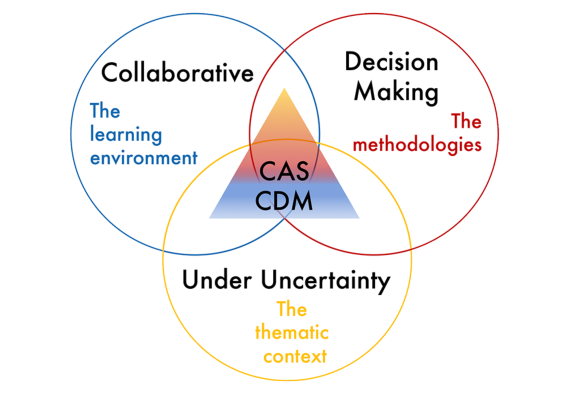
\includegraphics[scale=2.5]{Fig-circles}\\
{\small Figure 1: Method overview in 3  overlapping circles. } %% the captions 
\end{center}
%
Even the all-powerful Pointing \cite{Consonantia21} has no control about the blind texts it is an almost unorthographic life One day however a small line of blind text by the name of Lorem Ipsum decided to leave for the far World of Grammar. The Big Oxmox advised her not to do so, because there were thousands of bad Commas, wild Question Marks and devious Semikoli, but the Little Blind Text didn't listen.
} %% end text


% ====================== MATERIALS ===================
%% 
\def\materialstext
{\Large \black 
\begin{itemize}
\item Lorem ipsum dolor sit amet, consectetuer adipiscing elit. Aenean commodo ligula eget dolor. 
\item Aenean massa. Cum sociis natoque penatibus et magnis dis parturient montes, nascetur ridiculus mus. Donec quam felis, ultricies nec, pellentesque eu, pretium quis, sem.  
\end{itemize}
\vspace{6mm}
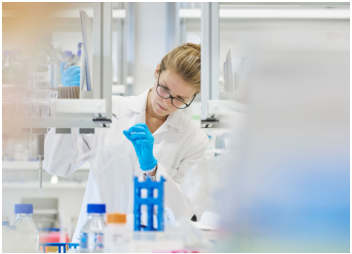
\includegraphics[scale=2.5]{Fig-Lab1}\quad 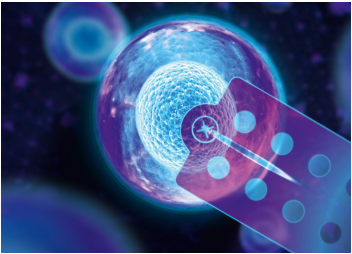
\includegraphics[scale=2.55]{Fig-Lab2}\\[-5mm] %%scale=2.5 forr landscape
{\small Figure 2: Pictures of lab staff and nanoscale experiment } %% the captions 

{\bf Again, take care of the resolution of your inserted pictures.} \\
She packed her seven versalia, put her initial into the belt.
}%% end text


% ====================== RESULTS / DISCUSSION ===================
%% 
\def\resultstext
{\Large \black 
Far far away, behind the word mountains, far from the countries Vokalia and Consonantia, there live the blind texts. Separated they live in Bookmarksgrove right at the coast of the Semantics, a large language ocean. A small river named Duden flows by their place and supplies it with the necessary regelialia. It is a paradisematic country, in which roasted parts of sentences fly into your mouth. 
\begin{center}
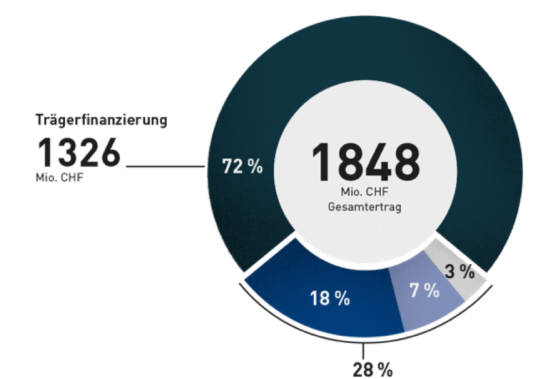
\includegraphics[scale=2.8]{Fig-Ring}\\[-5pt]
{\small Figure 3: Tr�gerfinanzierung in Prozentangaben im Ringdiagramm } %% the captions 
\end{center}



Even the all-powerful Pointing has no control about the blind texts it is an almost unorthographic life One day however a small line of blind text by the name of Lorem Ipsum decided to leave for the far World of Grammar.   \\
She packed her seven versalia, put her initial into the belt and made herself on the way. 
}%% end text


% ====================== CONCLUSION ===================
%% 
\def\conclusiontext
{\Large \black 
Here you present your conclusions in a short and easy to understand manner.
\begin{itemize}
\item Lorem ipsum dolor sit amet, consectetuer adipiscing elit. Aenean commodo ligula eget dolor. 
\item Cum sociis natoque penatibus et magnis dis parturient montes, nascetur ridiculus mus.
\end{itemize}
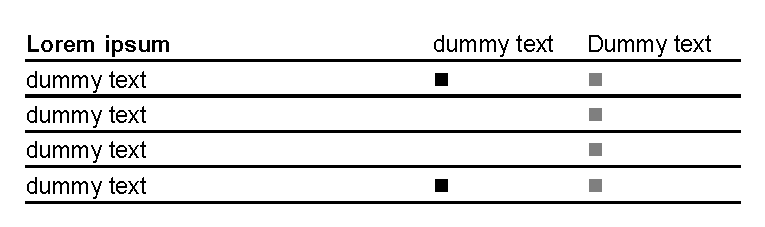
\includegraphics[scale=2.5]{Fig-Tabelle}

}%% end text



% ====================== REFERENCES ===================
%%
%%% you can use either your normal bib-file, insert file name
\def\bibfile{Poster-content}

%%% or you manually insert your references. In this case make sure to delete the \cite-entries in the dummy text.

\def\bibliotext
{\normalsize \black 
\begin{enumerate}
\item Lorem ipsum dolor sit amet, consectetuer adipiscing elit. Aenean commodo ligula eget dolor. 
\item Cum sociis natoque penatibus et magnis dis parturient montes, nascetur ridiculus mus. 
\end{enumerate}
}%% end text
